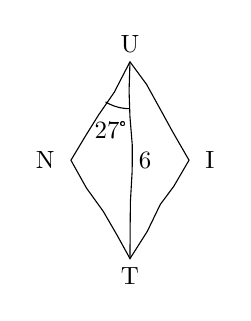
\begin{tikzpicture}[rotate=0,every node/.style={scale=0.9},scale=1]

\coordinate (N) at (0,0);
\coordinate (U) at (0.75,1.25);
\coordinate (I) at (1.5,0);
\coordinate (T) at (0.75,-1.25);

\draw[decorate,decoration={random steps,amplitude=1pt,segment length=10pt}] (N) node [left=3pt]{N}--(U) node [above]{U}--(I) node [right=3pt] {I}--(T) node [below] {T}--cycle;
\draw [decorate,decoration={random steps,amplitude=1pt,segment length=10pt}] (U)--(T);
\path (U)--(T) node[midway,right]{6};
\draw (0.44,0.74) arc (-120.96:-90:0.6) node[near start, below=3pt]{27°};

\end{tikzpicture}